\begin{figure}[htbp]
    \centering
    \footnotesize
    % First TikZ picture
    \begin{subfigure}[b]{0.45\textwidth}
        \centering
        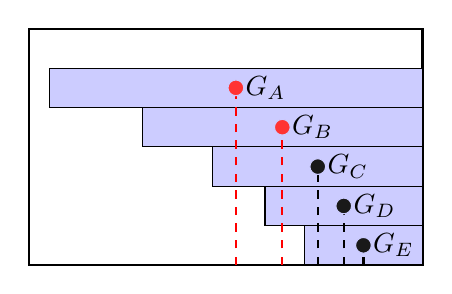
\begin{tikzpicture}
            % Draw the container
            \draw[thick] (0,0) rectangle (5,3);

            % Draw the three items inside
            % Draw the five items and their labels
            \draw[fill=blue!20] (3.5,0) rectangle (5,0.5);
            \draw[thick,dashed,black] (4.25,0) -- (4.25,0.25);  % <---
            \draw[fill = black!90, draw = blue!20] (4.25,0.25) circle (0.1);
            \node[anchor=west] at (4.25,0.25) {$G_E$};

            \draw[fill=blue!20] (3,0.5) rectangle (5,1);
            \draw[thick,dashed,black] (4,0) -- (4,0.75);  % <---
            \draw[fill = black!90, draw = blue!20] (4,0.75) circle (0.1);
            \node[anchor=west] at (4,0.75) {$G_D$};

            \draw[fill=blue!20] (2.33,1) rectangle (5,1.5);
            \draw[thick,dashed,black] (3.67,0) -- (3.67,1.25);  % <---
            \draw[fill = black!90, draw = blue!20] (3.67,1.25) circle (0.1);
            \node[anchor=west] at (3.67,1.25) {$G_C$};

            \draw[fill=blue!20] (1.44,1.5) rectangle (5,2);
            \draw[thick,dashed,red] (3.22,0) -- (3.22,1.75);  % <---
            \draw[fill=red!80, draw = blue!20] (3.22,1.75) circle (0.1);
            \node[anchor=west] at (3.22,1.75) {$G_B$};

            \draw[fill=blue!20] (0.26,2) rectangle (5,2.5);
            \draw[thick,dashed,red] (2.63,0) -- (2.63,2.25);  % <---
            \draw[fill=red!80, draw = blue!20] (2.63,2.25) circle (0.1);
            \node[anchor=west] at (2.63,2.25){$G_A$};


            %\node at (4, 1.875) {Fragile};
            %\node[anchor = west,align=center] at (2.9,2.5) {\small Center of \\  balance};

        \end{tikzpicture}
        \caption{Feasible, but unrobust, stacking with 75\% support area.}
    \end{subfigure}
    \hfill
    % Second TikZ picture
    \begin{subfigure}[b]{0.45\textwidth}
        \centering
        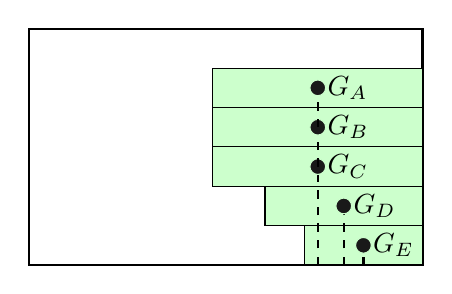
\begin{tikzpicture}
            % Draw the container
            \draw[thick] (0,0) rectangle (5,3);
            % Draw the three items inside
            % Draw the five items and their labels
            \draw[fill=green!20] (3.5,0) rectangle (5,0.5);
            \draw[thick,dashed,black] (4.25,0) -- (4.25,0.25);  % <---
            \draw[fill = black!90, draw = green!20] (4.25,0.25) circle (0.1);
            \node[anchor=west] at (4.25,0.25) {$G_E$};

            \draw[fill=green!20] (3,0.5) rectangle (5,1);
            \draw[thick,dashed,black] (4,0) -- (4,0.75);  % <---
            \draw[fill = black!90, draw = green!20] (4,0.75) circle (0.1);
            \node[anchor=west] at (4,0.75) {$G_D$};

            \draw[fill=green!20] (2.33,1) rectangle (5,1.5);
            \draw[thick,dashed,black] (3.67,0) -- (3.67,1.25);  % <---
            \draw[fill = black!90, draw = green!20] (3.67,1.25) circle (0.1);
            \node[anchor=west] at (3.67,1.25) {$G_C$};

            \draw[fill=green!20] (2.33,1.5) rectangle (5,2);
            \draw[thick,dashed,black] (3.67,1.25) -- (3.67,1.75);  % <---
            \draw[fill = black!90, draw = green!20] (3.67,1.75) circle (0.1);
            \node[anchor=west] at (3.67,1.75) {$G_B$};

            \draw[fill=green!20] (2.33,2) rectangle (5,2.5);
            \draw[thick,dashed,black] (3.67,1.75) -- (3.67,2.25);  % <---
            \draw[fill = black!90, draw = green!20] (3.67,2.25) circle (0.1);
            \node[anchor=west] at (3.67,2.25) {$G_A$};


            %\node at (4, 1.875) {Fragile};
            %\node[anchor = west,align=center] at (2.9,2.5) {\small Center of \\  balance};

        \end{tikzpicture}
        \caption{Feasible and robust stacking regarding 75\% support area.}
    \end{subfigure}
    \caption[Comparison of different vertical stability constraints.]{Comparison of different vertical stability constraints \\ with G = Center of Gravity (side view). \footnotemark}
    \footnotetext{Own figures based on \textcite[p. 845]{krebs_advanced_2021}.}
    \label{fig:vertical_stability_comparison}
\end{figure}
